\documentclass[12pt]{mwrep}
\usepackage{polski}
\usepackage[utf8]{inputenc}
\usepackage[T1]{fontenc}
\usepackage{times}



%\usepackage[margin=20mm, left=30mm]{geometry}

\usepackage{newtxtext}
\usepackage{newtxmath}
\usepackage{amsmath}
\usepackage{bm}
\usepackage{mathtools}
\mathtoolsset{showonlyrefs}


\usepackage{tabularx}
\usepackage{array}
\newcolumntype{Y}{>{\centering\arraybackslash}X}
\newcolumntype{Z}{>{\centering\arraybackslash}p}
\usepackage{multirow}
\usepackage{hyperref}

\usepackage{enumitem}
\usepackage{float}


\usepackage{graphicx}
\usepackage{rotating}
\usepackage{subcaption}


\usepackage{animate}

\renewcommand{\thesection}{\arabic{section}}
\renewcommand{\thesubsection}{\arabic{section}.\arabic{subsection}}


\begin{document}
	
	\begin{center}
		{\Large\textbf{Symulacje komputerowe}}
	\end{center}
	\begin{center}
		Raport 2
	\end{center}
	
	\noindent Temat: \ \textbf{\boldmath$\alpha$-stabilny proces L\'evy'ego}\\
	Imię i Nazwisko prowadzącego kurs: \ \textbf{Dr Michał Balcerek}	\newline\newline
	

	
	\noindent\begin{tabularx}{\textwidth}{|X |X|}
		\hline
		\begin{center}
			Imię i Nazwisko,\\nr indeksu
		\end{center} &  \begin{center}
			Kacper Budnik\\262286
		\end{center}\\\hline
		Wydział: & Wydział matematyki, W13 \\\hline
		Termin zajęć: & Wtorek,\vphantom{ $11^{1^{5}}$} $11^{15}$\\\hline
		Kod grupy ćwiczeniowej: & T00-70d \\\hline
		Data oddania raportu: & \today \\\hline
		\textbf{Ocena końcowa} &\\\hline
	\end{tabularx}\newline\newline


	\noindent\textbf{Adnotacje i uwagi:}
	
	\newpage
	
	
%	\section{Wstęp}
%	\noindent Drugi raport z symulacji komputerowych został podzielony na dwa zadania. Celem pierwszego z nich było dopasowanie modelu Ryzyka do otrzymanych danych oraz oszacowanie prawdopodobieństwa ruiny w skończonym i nieskończonym czasie. W tym celu:
%	\begin{itemize}[leftmargin=10mm, label=\small$\bullet$]
%		\item Znaleźliśmy rozkład zmiennej losowej $X_i$ oznaczającej wielkość $i$-tej szkody.
%		\item Wyestymowaliśmy pozostałe parametry procesu:
%		\begin{enumerate}[leftmargin=10mm]
%			\item $\lambda$ -- intensywność jednorodnego procesu Poissona,
%			\item $\theta$ -- parametr odpowiedzialny za wysokość premii.
%		\end{enumerate}
%		\item Oszacowaliśmy prawdopodobieństwo ruiny dla czasu:
%		\begin{enumerate}[leftmargin=10mm]
%			\item skończonego przy pomocy metody Monte Carlo,
%			\item nieskończonego przy pomocy algorytmu Pollaczka-Chinczyna.
%		\end{enumerate}
%	\end{itemize}
%	\noindent Drugie zadanie polegało natomiast na oszacowaniu średniego czasu wyjścia ruchu Browna z zadanego przedziału w zależności od punktu startowego. Dodatkowo mieliśmy oszacować prawdopodobieństwo wyjścia przez dany koniec odcinka. Na koniec, przy pomocy pakietów matematycznych, dopasowaliśmy funkcję do wygenerowanych metodą Monte Carlo danych.

	
	\section{Zadanie 2}
	\subsection{Proces Wienera}
	\noindent Procesem Wienera (Ruchem Browna) nazywamy proces $\{W_t\}_{t\geqslant0}$, który spełnia następujące własności:
	\begin{itemize}[leftmargin=10mm, label=\small$\bullet$]%label=$\boldsymbol{\cdot}$]
		\item $W_0=0$,
		\item $W_t$ ma niezależne przyrosty,
		\item $W_t$ ma stacjonarne przyrosty,
		\item $W_t \sim \mathcal{N}(0, t)$,
		\item $W_t$ ma ciągłe trajektorie.
	\end{itemize}	
	\noindent \textbf{Algorytm}\\
	\noindent Naszym celem jest wygenerowanie wektora $\left[W_{t_0}, W_{t_1}, \dots, W_{t_n}\right]$, gdzie
%	\begin{equation*}
%		t_i=ih, \quad i=0,1,\dots,n, \quad h=T/n
%	\end{equation*}
	\begin{equation*}
		t_i=ih, \quad i\in\left[n\right]=\left\{0, 1, \dots, n\right\}, \quad h=T/n.
	\end{equation*}
%	\begin{equation*}
%		t_i=ih, \quad i\in\mathbb{N}_0^{\leqslant n}, \quad h=T/n.
%	\end{equation*}
	W tym celu stosujemy poniższy algorytm
	\begin{enumerate}[leftmargin=10mm]
		\item Generuj realizację zmiennych $\xi_i\text{ iid. }\mathcal{N}(0,1), \,i\in\left[n-1\right]$,
		\item $W_{t_0}=W\left(0\right)=0$,
		\item $W_{t_{i+1}} = W_{t_{i}}+\sqrt{h}\xi_i,\quad i\in\left[n-1\right].$%\in\mathbb{N}^{n}$.
	\end{enumerate}

	\subsection{Czas wyjścia}
	\noindent Czasem wyjścia tego procesu z ustalonego przedziału $[a, b]$ nazywamy zmienną
	\begin{equation*}
		\tau=\inf\left\{t\geqslant0:W_t\notin[a, b]\right\}.
	\end{equation*}
	Niech $\left\{B^x_t\right\}_{t\geqslant0}$ będzie ruchem Browna startującym z $x\in\mathbb{R}$. Zdefiniujmy teraz zmienną 
	\begin{equation*}
		\tau^x=\inf\left\{t\geqslant0:B^x_t\notin[a, b]\right\}.
	\end{equation*}
%	dla $x$ z przedziału $[a,b]$.
	 Łatwo można pokazać, że $B^{x+y}_t\in[a ,b] \iff B^x_t\in[a-y, b-y]$.
%	\\Ponieważ $W_t+x\in[a, b] \iff W_t\in[a-x, b-x]$ \\
%	$B^x_t\in[a,b]\iff B^y_t\in[a-x+y, b-x+y]$\\widzimy, że czas wyjścia nie zależy bezpośrednio od wyboru punktów $a$ oraz $b$, a od punktu początkowego oraz długości przedziału.
	Dodatkowo, ponieważ ruch Browna jest $\frac{1}{2}$-samopodobny ($W_t\overset{d}{=}\sqrt{\Delta}W_{t/\Delta}$), zachodzi równość
	\begin{equation*}
		B^x_t=W_t+x\overset{d}{=}\Delta W_{t/\Delta^2}+x = \Delta\left(W_{t/\Delta}-\frac{x}{\Delta}\right)=\Delta B^{x/\Delta}_{t/\Delta^2}.
	\end{equation*}
	Korzystając z tych dwóch własności można udowodnić, że
	\begin{equation*}
		\begin{split}
			\tau^x&\overset{d}{=}\inf\left\{\Delta^2\frac{t}{\Delta^2}\geqslant0:\Delta B^{x/\Delta}_{t/\Delta^2}\notin[a, b]\right\} =\Delta^2\inf\left\{t^*\geqslant0:B^{x/\Delta}_{t^*}\notin\left[\frac{a}{\Delta},\frac{b}{\Delta}\right]\right\}\\
			&=\Delta^2\inf\left\{t^*\geqslant0:B^{(x-s)/\Delta}_{t^*}\notin\left[\frac{a-s}{\Delta},\frac{b-s}{\Delta}\right]\right\}.
		\end{split}
	\end{equation*}
	Wybierając teraz $\Delta=(b-a)$ oraz $s=a$ otrzymujemy
	\begin{equation}\label{eq:tau_przeskalowane}
		\tau^x\overset{d}{=}(b-a)^2\inf\left\{t\geqslant0:B^y_t\in[0,1]\right\}=(b-a)^2\widetilde\tau^y,
	\end{equation}
	gdzie $\widetilde\tau^y$ jest czasem wyjścia z przedziału $[0, 1]$, jeśli zaczniemy z punktu $y=\frac{x-a}{b-a}$, czyli z punktu dzielącego ten odcinek w stosunku takim samym jak $x$ dzieli odcinek $[a, b]$.\vspace{1.5mm}\\
	\noindent Dzięki tym przekształceniom widzimy, że $\mathbb{E}\tau^x$ zwiększa się z kwadratem długości przedziału jaki rozważamy oraz zależy ona od odległości $x$ od jednego końca przedziału względem drugiego. Z tego powodu później będziemy rozważać jedynie czas wyjścia z przedziału $[0, 1]$.
	
	
%	\subsection{Średni czas wyjścia procesu Wienera}
%%	\noindent Interesuje nasz średni czas wyjścia procesu w zależności od wybranego $x$. Można pokazać, że $\mathbb{E}\tau^x<\infty$\textsuperscript{\cite{art}}. Wiemy dodatkowo, że średnia w próbie jest dobrym estymatorem wartości oczekiwanej. Dlatego posłużyliśmy się tą metodą do oszacowania szukanej wartości. W wyniku otrzymaliśmy poniższy wykres
%	\noindent Interesuje nasz średni czas wyjścia procesu Wienera w zależności od wybranego punktu startowego $x$. Tą wielkość oszacowaliśmy poprzez obliczenie średniej w wygenerowanej przez nas próbie. Metoda jest poprawna, ponieważ średnia w próbie jest dobrym estymatorem wartości oczekiwanej oraz można udowodnić, że $\mathbb{E}\tau^x<\infty$\textsuperscript{\cite{art}}. W wyniku symulacji otrzymaliśmy poniższy wykres.
%%	 W wyniku otrzymaliśmy poniższy wykres
%	\begin{figure}[H]
%		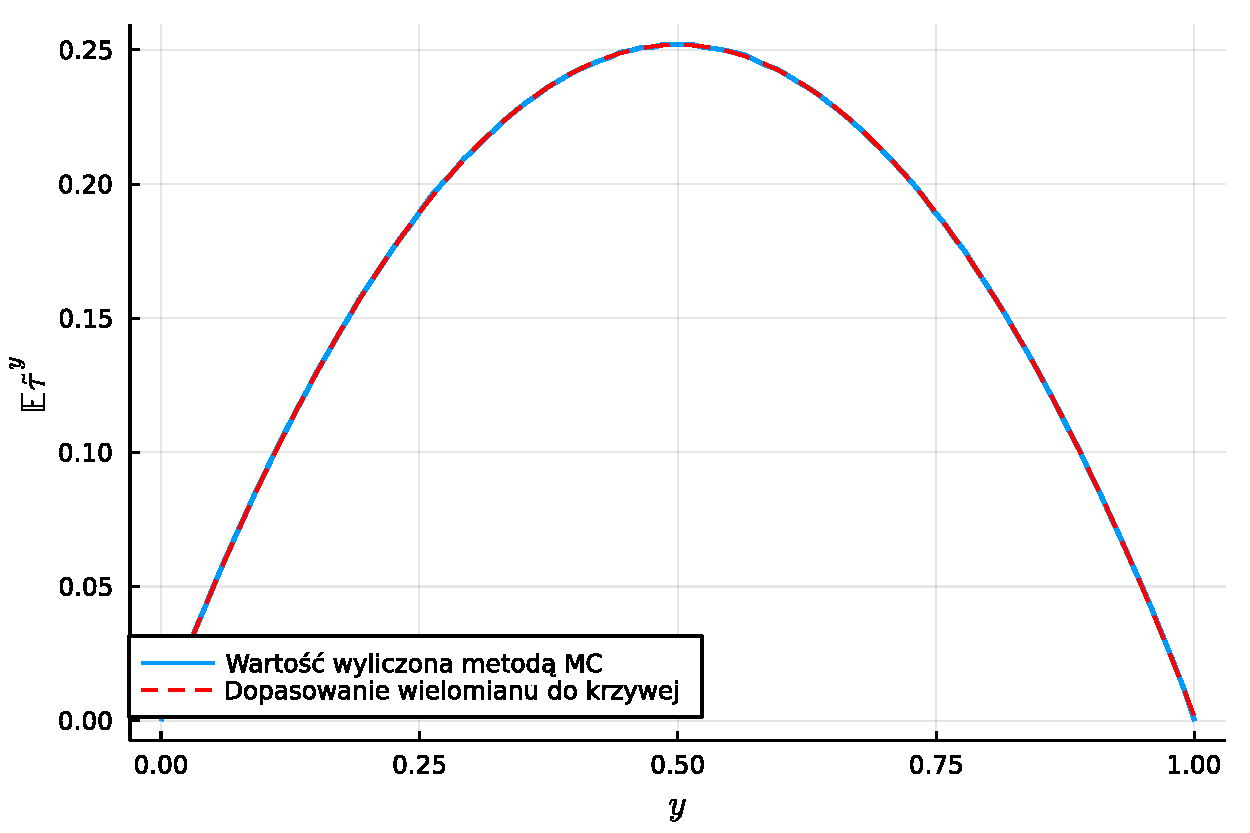
\includegraphics[width=\columnwidth]{fig/plot/expect_val.pdf}
%		\caption{Oszacowanie wartości oczekiwanej czasu wyjścia w zależności od punktu początkowego.}
%	\end{figure}
%%	\noindent Patrząc na wykres podejrzewaliśmy, że jest on wielomianem. Z pomocą pakietów matematycznych udało nam się dopasować funkcję $-1,0012y^2+1,0012y+0,0016$, która jak widzimy, dobrze przybliża otrzymaną krzywą.\\
%	\noindent Kształt wykresu mógł sugerować, że funkcja $f(y)=\mathbb{E}\widetilde\tau^y$ jest wielomianem. Z pomocą pakietów matematycznych udało nam się dopasować funkcję 
%	\begin{equation}\label{eq:oszac}
%		f(y)=-1,0012y^2+1,0012y+0,0016,
%	\end{equation}
%	która jak widzimy na wykresie, dobrze przybliża otrzymaną krzywą.\vspace{1.5mm}\\
%	Wartość oczekiwana czasu wyjścia dla standardowego procesu Wienera jest znana\textsuperscript{\cite{art}}
%%	Znana jest dokłada wartość wyjścia dla procesu Wienera\textsuperscript{\cite{art}}
%	\begin{equation*}
%		\mathbb{E}\mathbb{\tau}=ab,
%	\end{equation*}
%	gdzie $\tau$ jest czasem wyjścia z przedziału $[-a, b]$. Stąd, uwzględniając przesunięcie początkowe naszego procesu, otrzymujemy
%	\begin{equation*}
%		\mathbb{E}\widetilde\tau^y=y(1-y).
%	\end{equation*}
%	Stosując niewielkie przybliżenie (do 2-giego miejsca po przecinku) do funkcji \eqref{eq:oszac}, otrzymujemy wartość teoretyczną. Dodatkowo, korzystając teraz z \eqref{eq:tau_przeskalowane} oraz $y=(x-a)/(b-a)$ możemy uogólnić wzór na dowolny przedział $[a, b]$, otrzymując
%	\begin{equation*}
%		\mathbb{E}\tau^x=(b-a)^2\frac{x-a}{b-a}\left(1-\frac{x-a}{b-a}\right)=-(x-b)(x-a).
%	\end{equation*}
%
%%	Wynik otrzymany przez nasz nie różni się bardzo od wyniku analitycznego 
%	
%	\subsection{Prawdopodobieństwo wyjścia przez b}
%	\noindent Chcieliśmy jeszcze sprawdzić, jak często wyjście nastąpi przez większy z końców przedziału, czyli%większą z wartości końców przedziału, czyli
%	\begin{equation*}
%		\mathbb{P}\left(B^x_{\tau^x}=b\right).
%	\end{equation*}
%%	Korzystając z własności udowodnionych wcześniej oraz wykorzystując, że zmienna $B^x_{\tau^x}$ ma rozkład dwupunktowy skupiona na $\{a, b\}$, możemy prosto przekształcić to prawdopodobieństwo do postaci
%	Korzystając z własności udowodnionych wcześniej, przekształciliśmy powyższy wzór do postaci%możemy prosto przekształcić to prawdopodobieństwo do postaci
%	\begin{equation*}
%		\mathbb{P}\left(B^y_{\widetilde\tau^y}=1\right),
%	\end{equation*}
%	gdzie $\widetilde\tau^y$ jest czasem wyjścia procesu z przedziału $[0, 1]$. By oszacować to prawdopodobieństwo, ponownie skorzystaliśmy z metody Monte Carlo. Niestety generując trajektorię procesu generujemy punkty dyskretne, sprawdzając czy w danym momencie $B^x_t\geqslant b$. Prawdopodobieństwo, że trafimy dokładnie w punkt $b$ jest zatem znikome. Ponieważ $B^x_{\tau^x}$ może przyjmować jedynie dwie wartości, $a$ oraz $b$ ($b>a$), możemy przekształcić to prawdopodobieństwo, otrzymując
%	\begin{equation}\label{eq:dyskretyzaction}
%		\mathbb{P}\left(B^x_{\tau^x}=b\right)=\mathbb{P}\left(B^y_{\widetilde{\tau}^y}\geqslant1\right).
%	\end{equation}
%	 Wykorzystując powyższy wzór, byliśmy w stanie wygenerować poniższy wykres.
%	\begin{figure}[H]
%		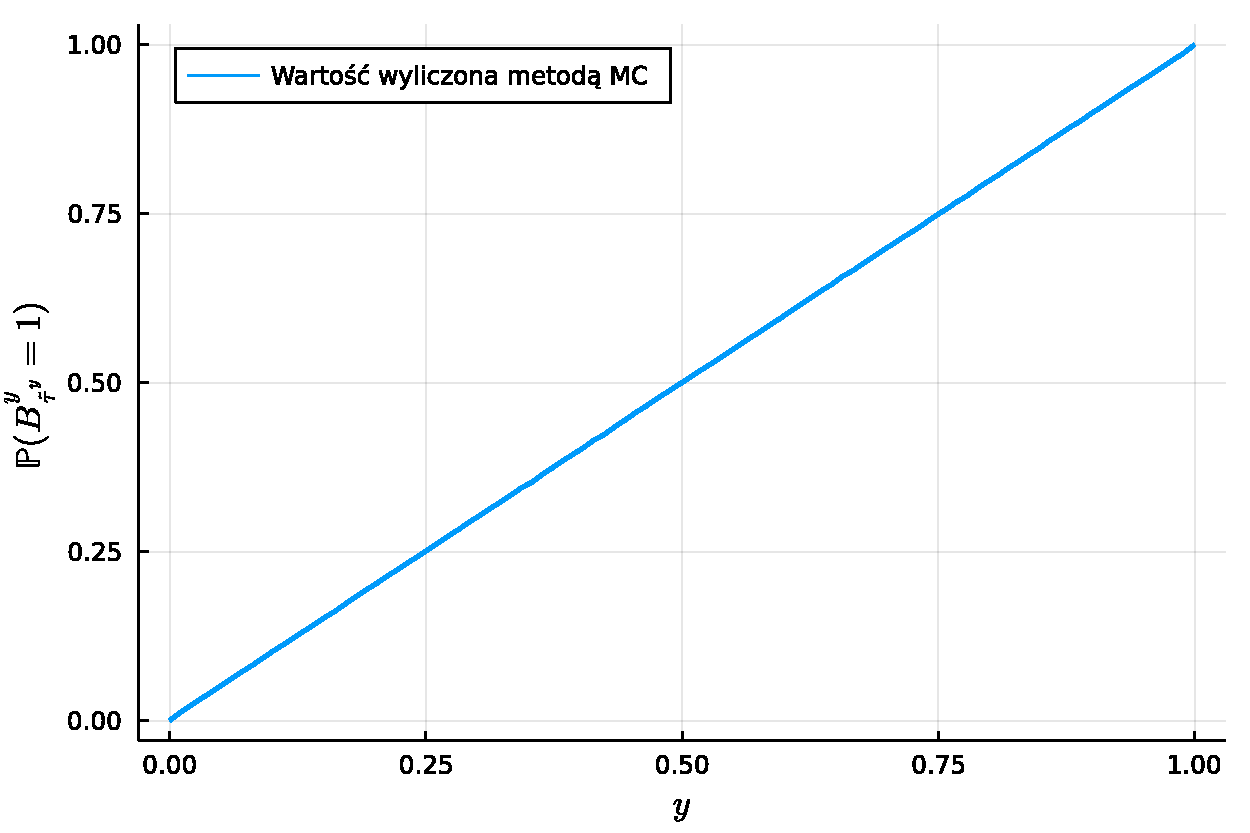
\includegraphics[width=\columnwidth]{fig/plot/prob.pdf}
%		\caption{Prawdopodobieństwo wyjścia przez punkt 1.}
%	\end{figure}
%	\noindent Na wykresie widoczna jest zależność liniowa $\mathbb{P}\left(B^y_{\widetilde{\tau}^y}\geqslant1\right) = y$ dla $y\in[0, 1]$. Korzystając z równości \eqref{eq:dyskretyzaction} oraz $y=(x-a)/(b-a)$ , szukane prawdopodobieństwo możemy przybliżać funkcją
%	\begin{equation}\label{eq:zad2_res}
%		\mathbb{P}\left(B^x_{{\tau}^x}= b\right)=\frac{x-a}{b-a}.
%	\end{equation}
%	Podobnie jak przy wyznaczaniu wartości oczekiwanej, znany jest nam wynik analityczny\textsuperscript{\cite{art}} dla procesu Wienera startującego w 0
%	\begin{equation*}
%		\mathbb{P}\left(W_{\tau}=b\right)=\frac{a}{b+a},
%	\end{equation*}
%	gdzie $\tau$ to czas wyjścia tego procesu z przedziału $[-a, b]$. Uwzględniając przesunięcie punktu początkowego szukane przez nas prawdopodobieństwo wynosi dokładnie
%	\begin{equation*}
%			\mathbb{P}\left(B^x_{\tau^x}=b\right)=\mathbb{P}\left(W_{\tau}=b-x\right)=\frac{x-a}{(b-x)+(x-a)}=\frac{x-a}{b-a}.
%	\end{equation*}
%	Powyższy wzór pokrywa ze wzorem \eqref{eq:zad2_res} uzyskanym przy pomocy symulacji.
%	\begin{equation*}
%		\mathbb{P}\left(B^x_{\tau^x}=b\right)=\mathbb{P}\left(B^y_{\widetilde\tau^y}=1\right)=\frac{y}{1-y+y}=y,
%	\end{equation*}
%	więc wyniki naszej symulacji pokrywają się z rozwiązaniami analitycznymi.



	\section{Zadanie 2 $\alpha$-stabilnych procesów L\'evy'ego}
	\noindent Procesem L\'evy'ego nazywamy proces $\{X_t: t\geqslant 0\}$, który\textsuperscript{\cite{Levy_def}}
	\begin{enumerate}[label=\textbf{(\roman*)}, leftmargin=10mm]
		\item trajektorie $X_t$ są $\mathbb{P}$- prawie na pewno prawostronnie ciągłe z lewostronnymi granicami,
		\item $\mathbb{P}\left(X_0=0\right)=1$,
		\item $X_t$ ma niezależna przyrosty,
		\item $X_t$ ma stacjonarne przyrosty.
	\end{enumerate}
	W tym raporcie będziemy badali czas wyjścia procesu L\'evy'ego $X_t^x=X_t+x$, takiego, że 
	\begin{equation}\label{X_dist}
		X_t\sim S_\alpha(t^{1/\alpha},0,0).
	\end{equation}
	Dla zadanego przedziału $[a, b]$ zdefiniujmy jeszcze zmienną
	\begin{equation}
		\tau^x=\inf\left\{t\geqslant0: X_t^x\notin[a,b]\right\},
	\end{equation}
	Oznaczającą czas wyjścia z zadanego przedziału w zależności od punktu startowego.\vspace{1.5mm}\\
	Łatwo można pokazać, że $X^{x+y}_t\in[a ,b] \iff X^x_t\in[a-y, b-y]$. Dodatkowo, ponieważ $X_t$ ma rozkład \eqref{X_dist}, to dla $a>0$ zachodzi
	\begin{equation}
		X_{at} \overset{d}{=} S_\alpha\left(\left(at\right)^{1/\alpha},0,0\right)\overset{d}{=}a^{1/\alpha}S_\alpha\left(t^{1/\alpha},0,0\right)
		\overset{d}{=}a^{1/\alpha}X_t,
	\end{equation}
	zatem proces $X_t$ jest procesem $1/\alpha$ podobnym. Teraz możemy pokazać poniższą równość.
	\begin{equation}
		X^x_t=X_t+x\overset{d}{=}\Delta X_{t/\Delta^{\alpha}}+x = \Delta\left(X_{t/\Delta^{\alpha}}-\frac{x}{\Delta}\right)=\Delta X^{x/\Delta}_{t/\Delta^\alpha}.
	\end{equation}
	 Korzystając z tych własności można pokazać, że
	\begin{equation}
		\begin{split}
		\tau^x&\overset{d}{=}\inf\left\{\Delta^\alpha\frac{t}{\Delta^\alpha}\geqslant0:\Delta X^{x/\Delta}_{t/\Delta^\alpha}\notin[a, b]\right\} 	=\Delta^\alpha\inf\left\{t^*\geqslant0:X^{x/\Delta}_{t^*}\notin\left[\frac{a}{\Delta},\frac{b}{\Delta}\right]\right\}\\
		&=\Delta^\alpha\inf\left\{t^*\geqslant0:X^{(x-s)/\Delta}_{t^*}\notin\left[\frac{a-s}{\Delta},\frac{b-s}{\Delta}\right]\right\}.
		\end{split}
	\end{equation}
	Wybierając teraz $\Delta=(b-a)$ oraz $s=a$ otrzymujemy
	\begin{equation}\label{eq:tau_przeskalowane}
		\tau^x\overset{d}{=}(b-a)^\alpha\inf\left\{t\geqslant0:B^y_t\in[0,1]\right\}=(b-a)^\alpha\widetilde\tau^y,
	\end{equation}
	gdzie $\widetilde\tau^y$ jest czasem wyjścia z przedziału $[0, 1]$, jeśli zaczniemy z punktu $y=\frac{x-a}{b-a}$, czyli z punktu dzielącego ten odcinek w stosunku takim samym jak $x$ dzieli odcinek~$[a, b]$.\vspace{1.5mm}\\
	\noindent Dzięki tym przekształceniom widzimy, że $\mathbb{E}\tau^x$ zależy od odległości $x$ od jednego końca przedziału względem drugiego oraz długości rozważanego odcinka. Ponieważ wiemy już jak wpływa ta długość na szukaną wartość oczekiwaną, będziemy rozważać jedynie czas wyjścia z przedziału $[0, 1]$.
	








%	
%	\section{Podsumowanie}
%	\noindent W zadaniu 1, korzystając z różnych metod statystycznych, udało nam się dopasować model klasycznego procesu Ryzyka do danych, co potwierdziło między innymi porównanie funkcji średniej procesu ze średnią z trajektorii z danych. Następnie wykorzystaliśmy wyznaczony model do oszacowania prawdopodobieństwa ruiny. Dokonaliśmy tego korzystając z metody Monte Carlo, a w przypadku nieskończonego czasu, ogromnie przydatny okazał się wzór Pollaczka-Chinczyna. Zgodnie z intuicją okazało się, że wraz ze zwiększaniem czasu, prawdopodobieństwo ruiny rośnie, jednak nie może przekroczyć tego dla nieskończonego czasu.\vspace{1.5mm}\\
%	\noindent Celem drugiego zadania było oszacowanie dwóch funkcji.
%	Zanim do tego przystąpiliśmy, pokazaliśmy, że rozpatrywany przedział mogliśmy wybrać swobodnie. W prosty sposób można uogólnić otrzymane wyniki na dowolny inny przedział. Obie funkcje oszacowaliśmy metodą Monte Carlo. W ten sposób otrzymaliśmy szukane funkcje
%	\begin{equation*}
%		\mathbb{E}\tau^x=-(x-b)(x-a)\quad\text{ oraz }\quad\mathbb{P}\left(B^x_{\tau^x}=b\right)=\frac{x-a}{b-a}.
%	\end{equation*}
%	Otrzymane wyniki bardzo dobrze odzwierciedlają wartości teoretyczne.\vspace{1.5mm}\\
%	\noindent Dodatkowo podczas symulacji zauważyliśmy, jak ważne jest generowanie procesu Wienera z odpowiednio małym krokiem czasowym. Wraz ze wzrostem wielkości kroku, rósł średni czas wyjścia procesu. By uzyskać dokładne dane, generowaliśmy proces z krokiem $h=10^{-4}$.
%	
%	
	
	
	
	
	\newpage
	\begin{thebibliography}{1}
		\bibitem{Levy_def}
		\url{https://people.bath.ac.uk/ak257/LCSB/part1.pdf}
		\bibitem{art}
		\url{https://galton.uchicago.edu/~lalley/Courses/313/BrownianMotionCurrent.pdf}
	\end{thebibliography}


\end{document}